\chapter{\label{chap:intro}Introdução}

Em 2014, 54\% da população mundial vivia em áreas urbanas, de acordo com a Organização das Nações Unidas~\cite{UN14}. A expectativa é que esta proporção aumente para 66\% até o ano 2050. Em números absolutos isto representa um acréscimo de 2,5 bilhões de pessoas à população urbana mundial nos próximos 35 anos. Uma das consequências da alta densidade populacional em regiões geográficas limitadas é o crescimento do modelo de verticalização na construção civil. Neste cenário, onde prédios de diversos andares se tornam presença no cotidiano da maioria da população, os elevadores passam a um papel de destaque.

Uma pesquisa realizada pela IBM no ano de 2010 em 16 cidades norte-americanas constatou que, durante 12 meses, o tempo acumulado no qual trabalhadores de escritórios\footnote{Em uma força de trabalho total de 51 milhões de trabalhadores, dos quais 12,7 milhões são usuários de elevadores diariamente~\cite{IBM10}.} aguardaram por elevadores foi de 92 anos~\cite{IBM10}. Em uma economia onde o salário horário médio de um trabalhador é de US\$ 24,99, o tempo de espera por elevadores representa custos de mais de US\$ 20 bilhões em média por ano~\cite{BLS15}.

Além do impacto econômico existe o impacto psicológico. Trabalhadores em centros metropolitanos empreendem uma parcela significativa da sua rotina no deslocamento entre residência e local de trabalho e no caminho inverso ao final do dia. Além de gastar uma quantidade significativa de tempo no trânsito das ruas, em carros, ônibus, bicicletas e metrôs, o tempo compreendido entre aguardar o elevador e desembarcar no andar desejado está longe de ser desprezível. Em função disso, ajustam sua rotina abrindo mão de momentos de momentos de descanso ou lazer. Uma possível consequência é um aumento nos níveis de estresse e um decréscimo na qualidade de vida a médio e longo prazo. {\color{red}[BUSCAR FONTES PARA ESTE PARÁGRAFO]} % TODO: CITATIONNEEDED

\begin{figure}[htb!]
\centering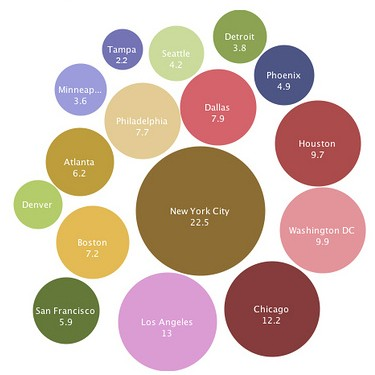
\includegraphics{img/time-cost.jpg}
\caption{\label{fig:fig1}Tempo de espera acumulado (em anos) por elevadores durante 12 meses em 16 cidades norte-americanas. Fonte:~\cite{IBM10}}
\end{figure}

Neste contexto global, a indústria de elevadores possui alguns desafios: primeiro, lidar com a pressão para a redução de custos na construção civil, construindo elevadores mais baratos e eficientes, com melhorias no desempenho de transporte; segundo, competir no mercado oferecendo serviços novos, personalizados e com garantia de qualidade, visando revolucionar a maneira com que elevadores interagem e servem passageiros~\cite{KOEHLEROTTIGER02}. Já sob o ponto de vista dos passageiros, estes esperam que suas chamadas sejam atendidas imediatamente e que sejam levados ao seu destino o mais rápido possível.

Existem diversas abordagens que os fabricantes de elevadores podem usar para minimizar o tempo de espera, como aumentar o número de elevadores no prédio ou a capacidade de cada elevador. Entretanto, este tipo de alteração não é sempre realizável em função de limitações na estrutura do prédio ou inviabilidade financeira. Como alternativa e muitas vezes uma solução de mais fácil aplicação é otimizar o sistema de controle dos elevadores. Ainda assim, a tarefa de atribuir elevadores para atender chamadas minimizando o tempo médio de espera está no conjunto de problemas NP-difícil (ou NP-hard, ou NP-complexo)~\cite{SeKo99}. Portanto, uma solução ótima para este problema ainda não é conhecida.

Desde meados dos anos 1980, a indústria de elevadores vem estudando e implementando estratégias para encontrar soluções sub-ótimas para o problema. Diversas técnicas de Inteligência Artificial foram adotadas, como redes neurais, algoritmos genéticos, lógicas \textit{fuzzy} e, mais recentemente, sistemas multi-agentes, planejamento e aprendizado de máquina~\cite{KOEHLEROTTIGER02}.

A proposta deste trabalho é comparar diferentes estratégias de controle de elevadores em alguns cenários e avaliar, dentre as opções possíveis, quais combinações resultam em um melhor desempenho no transporte de passageiros. A comparação se dará analisando os resultados de simulações de diferentes algoritmos de controle.

Para tanto, serão implementados no mínimo 2 algoritmos para o sistema de controle de elevadores e um simulador de elevadores. O usuário do simulador poderá:

\begin{itemize}
  \item Selecionar cenários;
  \item Selecionar um algoritmo para controle dos elevadores ou implementar o seu próprio;
  \item Comparar o desempenho entre diferentes algoritmos em um mesmo cenário;
  \item Comparar o desempenho de um algoritmo em múltiplos cenários.
\end{itemize}

Com base nos resultados estatísticos obtidos através das simulações serão realizadas análises quantitativas e qualitativas e, se possível, otimizações nas implementações dos algoritmos. Assim, objetiva-se encontrar quais são as melhores estratégias para cada cenário proposto.

\section{Motivações}

\subsection{Motivação Prática}
O estudo de Inteligência Artifical é um grande interesse dos autores, junto dos
problemas relacionados a Simulação e às ferramentas de Programação. O problema
de alocação ótima e otimização do tempo de viagem de elevadores apresenta um
campo de pesquisa único para a aplicação destas ferramentas em busca da prática
da Inteligência Artificial.

Além disso, o uso de elevadores é uma constante na vida de todos os habitantes
de grandes metrópoles. Uma parcela significativa do dia-a-dia de todos nós é
passada em grandes caixas metálicas, ou esperando pelas mesmas. A possibilidade
de aplicarmos nossos conhecimentos em Inteligência Artificial para melhorar a
performance deste meio de transporte tão ubíquito e, por conseqüência, a
qualidade de vida de todos seus usuários é um grande atrativo para a escolha
deste tópico.

Desde sua concepção, houve pouca evolução nos elevadores. De fato, o mecanismo
que os faz mover evoluiu drasticamente, quando comparamos simples elevadores de
tração manual com as máquinas modernas que estão presentes nos mais novos
arranha-céus. No entanto, o sistema de controle dos mesmos ainda é um tanto
quanto arcaico, utilizando-se muito pouco de técnicas de aprendizado e
heurísticas para alterar seu comportamento em tempo de execução. Acreditamos que
seja possível trazer uma revolução tão grande para os sistemas de controle com
Inteligência Artificial quanto os motores elétricos foram para a tração dos elevadores.

Os problemas de Simulação também são particularmente interessantes. Definir
métricas e realizar a coleta de dados significativos para o problema é um
conjunto de habilidades que perdurará e será de inestimável valor profissional e pessoal.

\section{Glossário}

Termos chaves usados neste trabalho.

\begin{description}[leftmargin=!,labelwidth=\widthof{\bfseries Sistema de Controle}]
  \item[Lobby]                Andar térreo de um prédio.
  \item[Elevador]             Dispositivo de transporte vertical que movimenta pessoas ou cargas entre andares ou níveis de um prédio ou estrutura.
  \item[pickup call]          Chamada na qual passageiros estão fora dos elevadores e pressionam o botão (subir ou descer) do andar em que se encontram.
  \item[cabin call]           Chamada na qual passageiros estão dentro do elevador e pressionam o botão correspondente ao andar para o qual desejam ir.
  \item[Sistema de Controle]  O sistema central que gerencia todos os elevadores.
\end{description}